\section{Machine Control}

\begin{itemize}
\tightlist
\item
introduction, the democratization of automation
\item
structure of hypercube, workflow, general principles
\item
trash robot printer
\item
wall robot on large building
\item
agricultural robot prototype/description
\item
electron beam lithography
\item
hacked 3d printer to make 2.5d printer
\end{itemize}


\begin{figure}
	\centering
	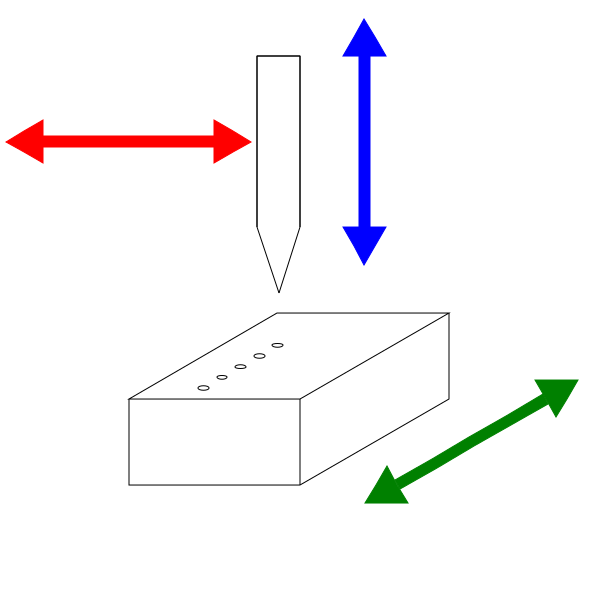
\includegraphics[width=4in]{figures/machines/xyzprobe.png}
	\caption[xyzprobe]
	{A probe move over a sample in either the x or z direction, and the sample moves along the y axis.  Repeated poking of the sample prints dots a simple but very versatile tool.}
\end{figure}


\begin{figure}
	\centering
	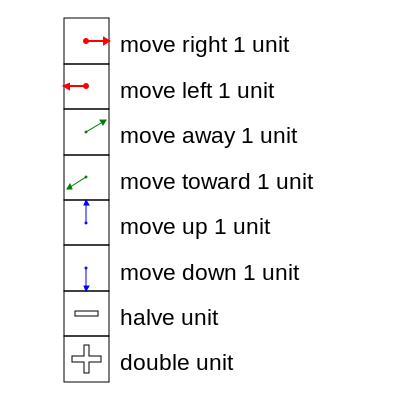
\includegraphics[width=4in]{figures/machines/basicmovements.png}
	\caption[basicmovements]
	{Basic geometric actions of machine control for an arbitrary machine that moves along three perpendicular axes.}
\end{figure}

\begin{figure}
	\centering
	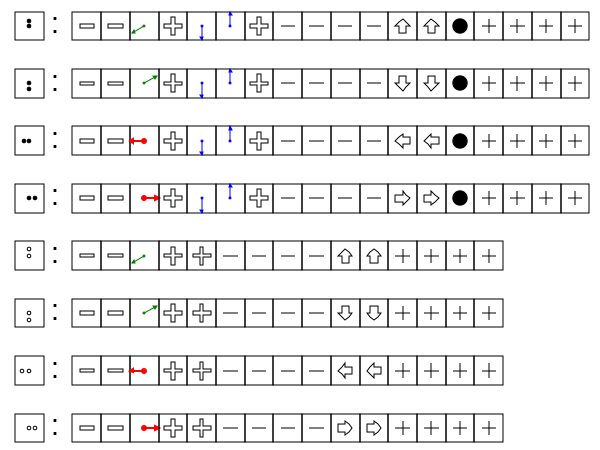
\includegraphics[width=4in]{figures/machines/actions05xx.png}
	\caption[actions05xx]
	{Dot actions from which symbols are constructed.}
\end{figure}


\begin{figure}
	\centering
	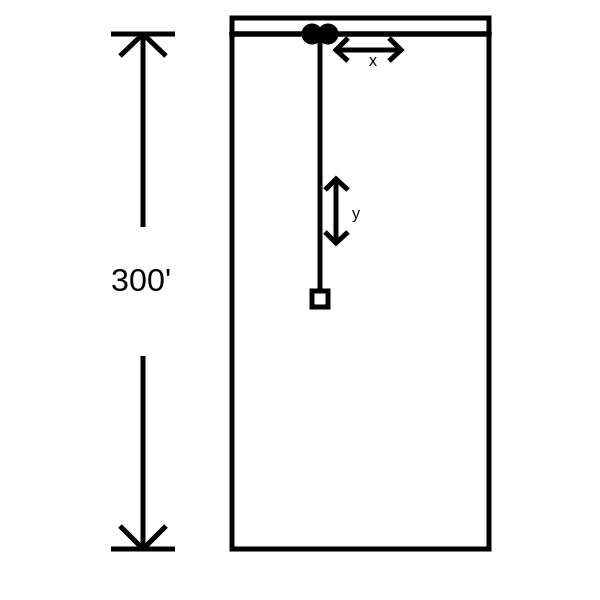
\includegraphics[width=4in]{figures/machines/buildingwallrobot.png}
	\caption[buildingwallrobot]
	{A hoist run along a rail going across the edge of a roof of a building can make a simple robot which can move to anywhere along the wall.}
\end{figure}
